127. \begin{figure}[ht!]
\center{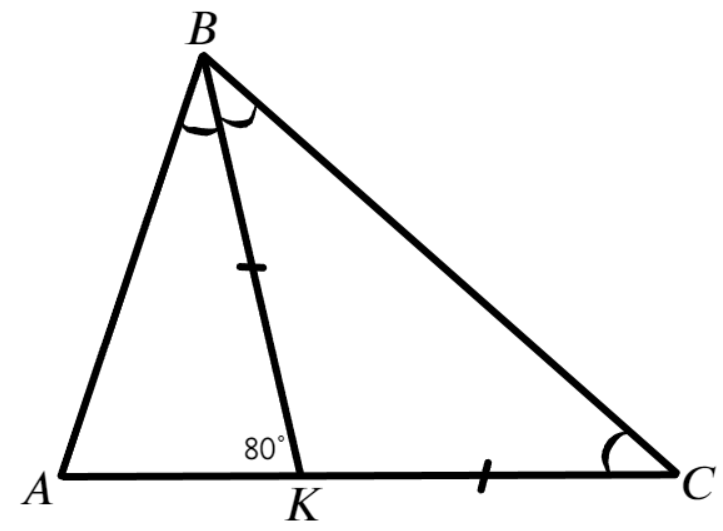
\includegraphics[scale=0.35]{g7-127.png}}
\end{figure}\\
Так как $BK$ является биссектрисой, обозначим $\angle ABK=\angle KBC=x.$ Так как $BK=KC,$ треугольник $KBC$ является равнобедренным и $\angle KCB=\angle KBC=x.$ Так как $\angle BKC=180^\circ-\angle AKB=180^\circ-80^\circ=100^\circ,$ имеем $x=(180^\circ-100^\circ):2=40^\circ.$ Тогда $\angle BAC=180^\circ-2x-x=180^\circ-120^\circ=60^\circ.$\\
